\section{Experimental Details}
\label{appendix:exp_details}
In this section, we present our experimental details, including dataset descriptions, implementation specifics, extended results, and additional analyses that complement our main findings.

\begin{algorithm}[tb]
\caption{Tool-calling with \method}
\label{alg:toolspec}
\small
\begin{algorithmic}[1]
\Require target model $\mathcal{M}$; input query $\boldsymbol{x}$; tool documentation $\mathcal{D}$; historical datastore $\mathcal{H}=\{(\boldsymbol{h}_j,\boldsymbol{y}_j)\}_{j=1}^{|\mathcal{H}|}$; parameter $k$.
\Ensure Generated tool-call sequence $\boldsymbol{y}$.

\State Parse documentation $\mathcal{D}$ into schema $\mathcal{S}$ %
\State Construct the FSM $\mathcal{F}=(\mathcal{Q}, \Sigma_{\text{schema}}, \delta, q_0)$ from $\mathcal{S}$
\State $\boldsymbol{y} \gets \emptyset$, $q \gets q_0$
\State Compute query representation $\boldsymbol{h}_x$
\State Retrieve historical calls $\mathcal{I}_k \gets \operatorname{Top-K}_{j} \text{sim}(\boldsymbol{h}_x,\boldsymbol{h}_j)$
\While{\textsc{NotFinished}$(q,\boldsymbol{y})$}
    \mydarkcolor{\LineComment{Retrieval-augmented speculation}}
    \State $\mathcal{B}_{\text{retrieval}} \gets \textsc{SuffixMatch}(\boldsymbol{y}, \{{\boldsymbol{y}}_{j}\}_{j \in \mathcal{I}_k})$
    \If{$\mathcal{B}_{\text{retrieval}} \neq \emptyset$}
        \State $\mathcal{B} \gets \mathcal{B}_{\text{retrieval}}$
    \Else
        \mydarkcolor{\DoubleLineComment{Schema-aware drafting}}
        \State $\mathcal{B} \gets 
        \textsc{SchemaAwareDraft}(q,\mathcal{S},\boldsymbol{y})$
    \EndIf
    \mydarkcolor{\LineComment{Packed sequence with tree attention}}
    \State $(\boldsymbol{z},\mathbf{A}) \gets \textsc{PackDraftsAsTree}(\mathcal{B})$
    \State $\hat{\mathcal{B}} \gets \textsc{Verification}(\mathcal{M}, \boldsymbol{x}, \boldsymbol{y}, \boldsymbol{z}, \mathbf{A})$
    \State $(\tilde{\boldsymbol{y}}^\star,\ell) \gets \textsc{SelectLongestAcceptedPrefix}(\hat{\mathcal{B}})$
    \State $\boldsymbol{y} \gets \boldsymbol{y} \oplus \tilde{\boldsymbol{y}}^\star_{1:\ell}$
    \mydarkcolor{\LineComment{Update FSM state}}
    \State $q \gets \delta(q, \tilde{\boldsymbol{y}}^\star_{1:\ell})$
\EndWhile

\State \Return $\boldsymbol{y}$
\end{algorithmic}
\end{algorithm}

\subsection{Datasets} 
\label{appendix:dataset_details}
Our evaluation encompasses four widely used tool-use benchmarks. The details of the evaluation data are illustrated as follows:
\begin{itemize}
    \item  \textbf{API-Bank}~\citep{apibank}: a three-level evaluation framework comprising 73 diverse APIs. It evaluates an LLM’s ability to select and invoke tools through natural multi-turn dialogues across varying levels of difficulty.
    \item  \textbf{ToolAlpaca}~\cite{ToolAlpaca}: a benchmark for assessing general-purpose tool-use capabilities of LLMs. The evaluation dataset consists of two subsets: (i) a simulated subset with 10 synthetic tools, and (ii) a real-world subset with 11 APIs from diverse domains.
    \item  \textbf{BFCLv2}~\cite{BFCL}: a comprehensive benchmark covering a wide range of scenarios, including single-step reasoning, multi-step tool use, real-time execution, etc. We evaluate \method under both single-function and multi-function settings.
    \item  \textbf{ToolBench}~\cite{Qin:2024toolllm}: a large-scale, high-quality benchmark featuring multi-tool and multi-turn interactions over 16,464 real-world APIs, automatically constructed using ChatGPT. We evaluate \method on its single-tool subset.
\end{itemize}

\subsection{Implementation Details} 
\label{appendix:impl_details}
The retrieval parameter $k$ is set to $10$, such that the top-$10$ candidates are retained at each retrieval step. For suffix matching, we follow PLD~\citep{saxena2023pld} and consider suffix lengths $L \in \{5,6,7\}$, applying a longest-first strategy (from $7$ to $5$). Once a match is found, we extract continuations following the matched suffix in sequential order, using predefined lengths $n \in \{32, 16, 8, 8\}$ to construct draft candidates. We adopt Token Recycling (TR)~\citep{luo:2025tokenrecycle} as the general speculative generation strategy in \method. All experiments were conducted using PyTorch 2.5.1 on 2$\times$NVIDIA A100-PCIE GPUs (40GB) with 40 CPU cores under CUDA 12.4. Inference for our method and all baselines was performed using the Hugging Face transformers package. Following prior work, we adopt speculative sampling~\citep{leviathan:2023spec} as our acceptance strategy, with a batch size of 1.

\subsection{Performance Comparison} 
\label{appendix:performance}
Table~\ref{tab:performance} illustrates the accuracy comparison between \method and vanilla autoregressive decoding across different models on API-Bank and ToolAlpaca. The results demonstrate that \method preserves the original performance of autoregressive decoding, achieving consistently comparable accuracy across various models and datasets. The slight discrepancy observed for Qwen2.5-14B on ToolAlpaca can be attributed to fp16 precision.

\begin{table}[t]
\centering
\small
\resizebox{\linewidth}{!}{
\begin{tabular}{@{}llccc@{}}
\toprule
\bf Models &\bf Methods & \bf API-Bank & \bf ToolAlpaca \\\midrule
\multirow{2}{*}{Qwen2.5-7B}
&Vanilla & 54.94 & 58.94 \\
&\method & \green{54.94} & \green{58.94} \\\midrule
\multirow{2}{*}{Qwen2.5-14B}
&Vanilla & 54.61 & 58.94 \\
&\method & \green{54.61} & \green{59.60} \\\midrule
\multirow{2}{*}{LLaMA-3.1-8B}
&Vanilla & 59.30 & 48.34 \\
&\method & \green{59.30} & \green{48.34} \\\midrule
\multirow{2}{*}{LLaMA-3.2-3B}
&Vanilla & 50.08 & 41.72 \\
&\method & \green{50.08} & \green{41.72} \\
\bottomrule
\end{tabular}}
\caption{Performance comparison between \method and vanilla autoregressive decoding across different models on two widely used tool-use benchmarks.}
\label{tab:performance}
\end{table}

\subsection{Hyperparameters in \method}
Table~\ref{tab:continuation} and Table~\ref{tab:topk} show the speedup of \method under different hyperparameter settings, including continuation length and the retrieval parameter $k$. The evaluation is conducted on 100 instances sampled from the training set of API-Bank~\citep{apibank}. Table~\ref{tab:continuation} shows that shorter continuation lengths (e.g., $\{16, 8, 4, 4\}$) lead to suboptimal \#MAT and speedup. Although longer continuation lengths (e.g., $\{64, 32, 16, 8\}$) slightly improve \#MAT, they also introduce additional computational overhead and reduce the overall speedup. Therefore, we adopt continuation lengths of $\{32, 16, 8, 8\}$ in our experiments. We further compare this setting with uniform continuation lengths of $\{16, 16, 16, 16\}$, and the results show that allocating longer continuations to top-ranked candidates brings greater benefits. Similarly, Table~\ref{tab:topk} shows that setting the retrieval parameter $k$ to 10 achieves the best speedup in our experiments.

\begin{table}[t]
\centering
\small
\begin{tabular}{@{}l|ccc@{}}
\toprule
\bf Continuations &\#MAT &Tokens/s & Speedup \\\midrule
$\{16, 8, 4, 4\}$ & 5.52 & 115.07 & 4.08$\times$  \\
$\{32, 16, 8, 8\}$ & 5.75 & \bf{124.77} & \bf{4.42$\times$} \\
$\{64, 32, 16, 8\}$ & \bf{5.77} & 122.60 & 4.35$\times$ \\
$\{16, 16, 16, 16\}$ & 5.60 & 117.95 & 4.18$\times$  \\
\bottomrule
\end{tabular}
\caption{Speedup of \method under different continuation lengths. Results are obtained with LLaMA-3.1-8B-Instruct on API-Bank.}
\label{tab:continuation}
\end{table}

\begin{table}[t]
\centering
\small
\begin{tabular}{@{}l|ccc@{}}
\toprule
\bf $k$ &\#MAT &Tokens/s & Speedup \\\midrule
$1$ & 5.13 & 113.18 & 4.01$\times$  \\
$5$ & 5.56 & 119.70 & 4.24$\times$ \\
$10$ & \bf{5.75} & \bf{124.77} & \bf{4.42$\times$} \\
$15$ & 5.69 & 123.22 & 4.37$\times$  \\
\bottomrule
\end{tabular}
\caption{Speedup of \method with different retrieval parameter values $k$. Results are obtained with LLaMA-3.1-8B-Instruct on API-Bank.}
\label{tab:topk}
\end{table}

\subsection{Memory Cost}
The additional memory overhead introduced by \method is modest. The primary persistent cost comes from the \textit{output memory}, which stores the hidden state of each input question,  along with its corresponding output tokens for each memorized sample. On API-Bank, this memory requires only 4.9 MB for 597 entries, corresponding to approximately 0.0082 MB per entry. To support larger datasets, \method can maintain a fixed-size memory bank, such as 1,000 memorized samples, thereby bounding the output memory while preserving the benefits of retrieval-augmented speculation. We leave the design of such memory management strategies for future investigation.

\begin{table}[t]
\centering
\small
\begin{tabular}{@{}l|ccc@{}}
\toprule
\textbf{Models} &\#MAT &Tokens/s & Speedup \\\midrule
Vanilla & 1.00 & 17.23 & 1.00$\times$  \\
PLD & 1.91 & 28.24 & 1.64$\times$ \\
TR & 2.90 & 30.30 & 1.76$\times$ \\
SAMD & \underline{2.99} & \underline{30.73} & \underline{1.78$\times$}  \\
\method & \bf{4.72} & \bf{52.42} & \bf{3.04$\times$}  \\
\bottomrule
\end{tabular}
\caption{Speedup of \method and prior plug-and-play methods using Qwen2.5-32B-Instruct on API-Bank. The best results are shown in \textbf{boldface}, and the second-best results are \underline{underlined}.}
\label{tab:32b}
\end{table}

\begin{figure}[t]
\centering
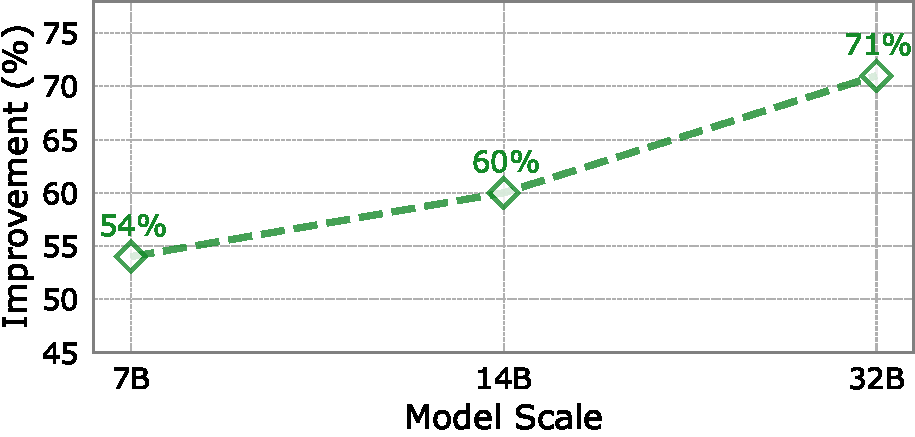
\includegraphics[width=0.95\columnwidth]{fig/scaling.pdf}
\caption{Relative speedup improvement of \method over the previous best method. Results are obtained using the Qwen series on API-Bank.}
\label{fig:scaling}
\end{figure}

\subsection{Results on Qwen2.5-Instruct-32B}
\label{appendix:qwen32B}
Table~\ref{tab:32b} compares the speedup of \method with prior plug-and-play methods on API-Bank using Qwen2.5-32B-Instruct. The results demonstrate that \method outperforms these baselines and achieves up to a $3\times$ speedup over standard autoregressive decoding. Figure~\ref{fig:scaling} shows that the relative speedup gain of \method over the strongest reproduced baseline becomes larger as the model size increases. These results suggest that \method scales favorably with model size and provides increasingly pronounced efficiency benefits over existing plug-and-play approaches.

\begin{figure}[t]
\centering
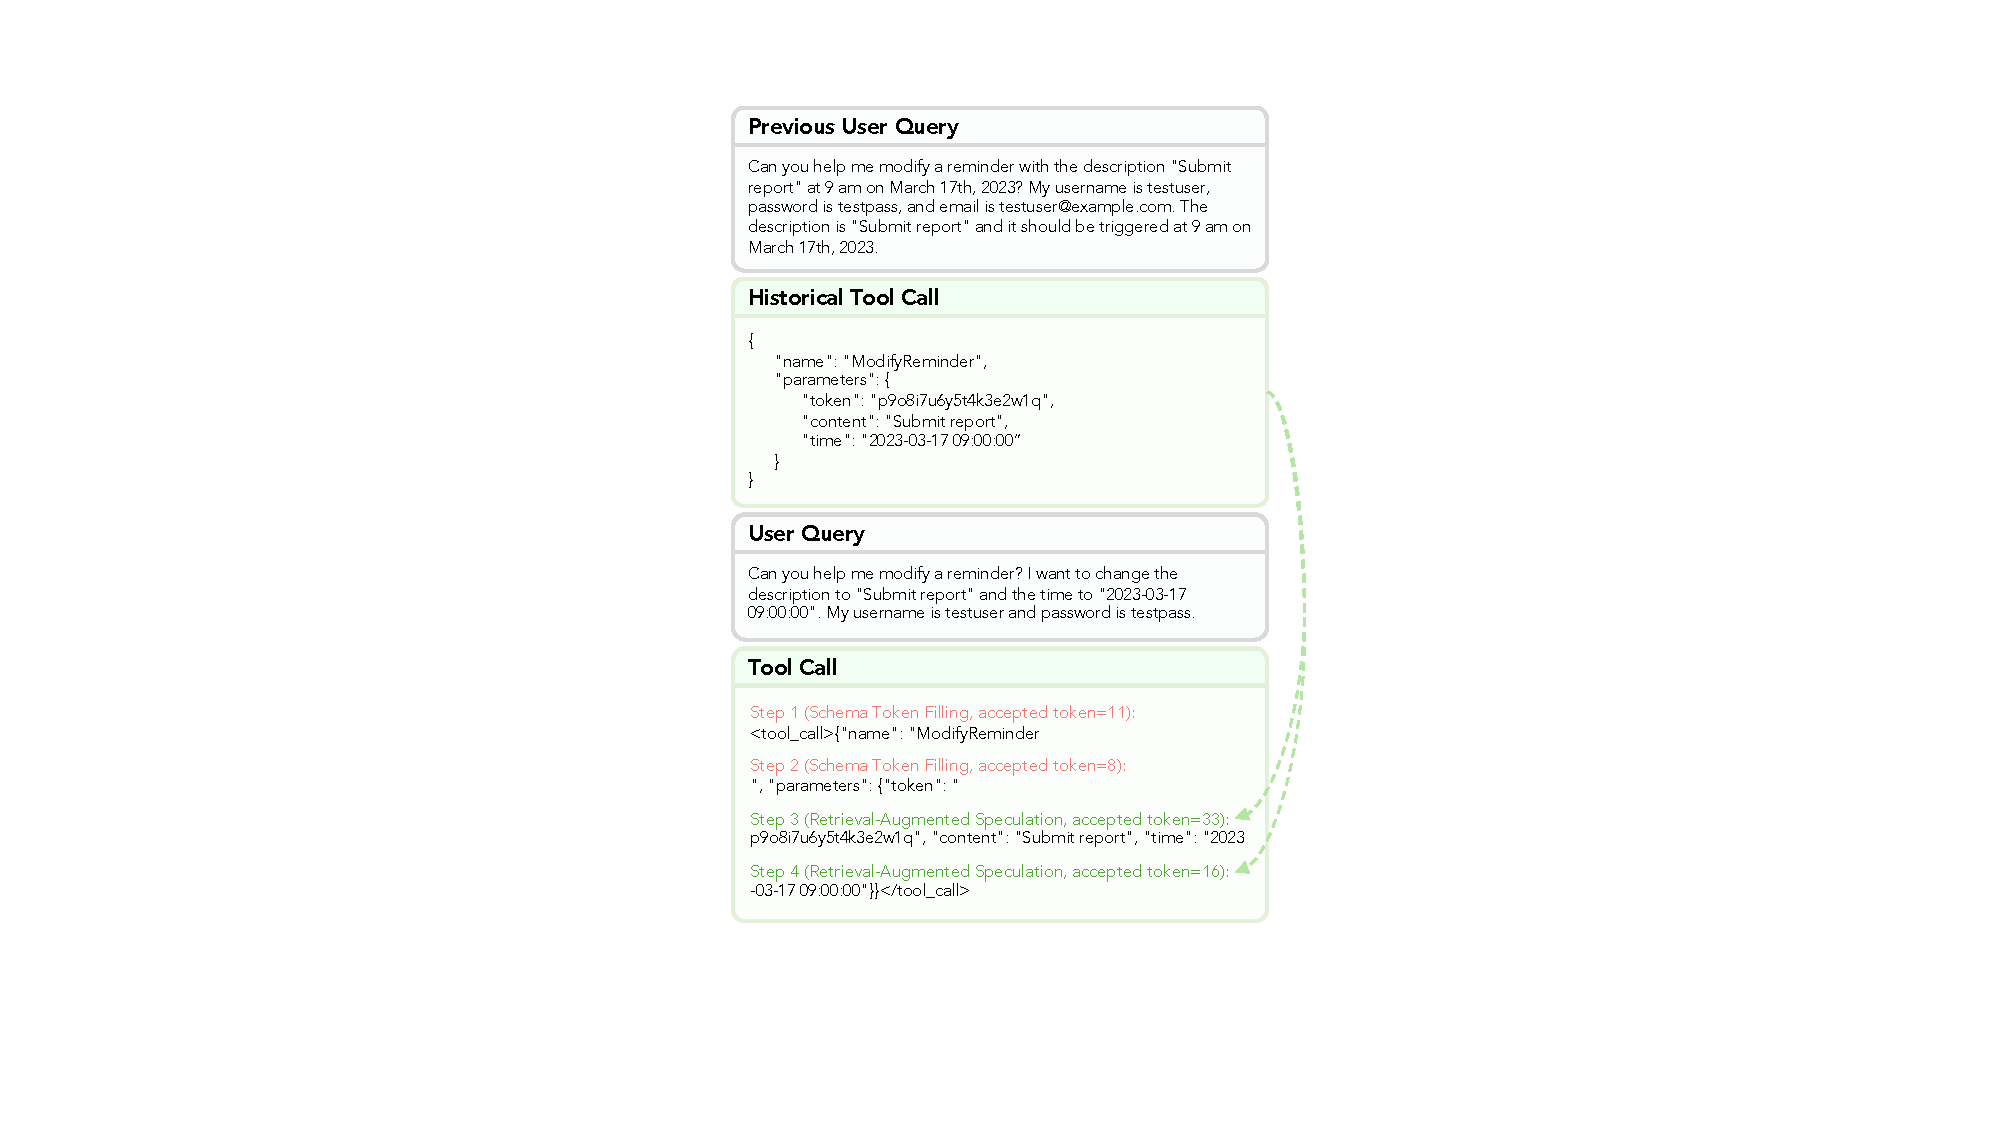
\includegraphics[width=0.95\columnwidth]{fig/case1.pdf}
\caption{Case study of \method with similar user queries on API-Bank using LLaMA-3.1-8B-Instruct.}
\label{fig:case1}
\end{figure}

\begin{figure}[t]
\centering
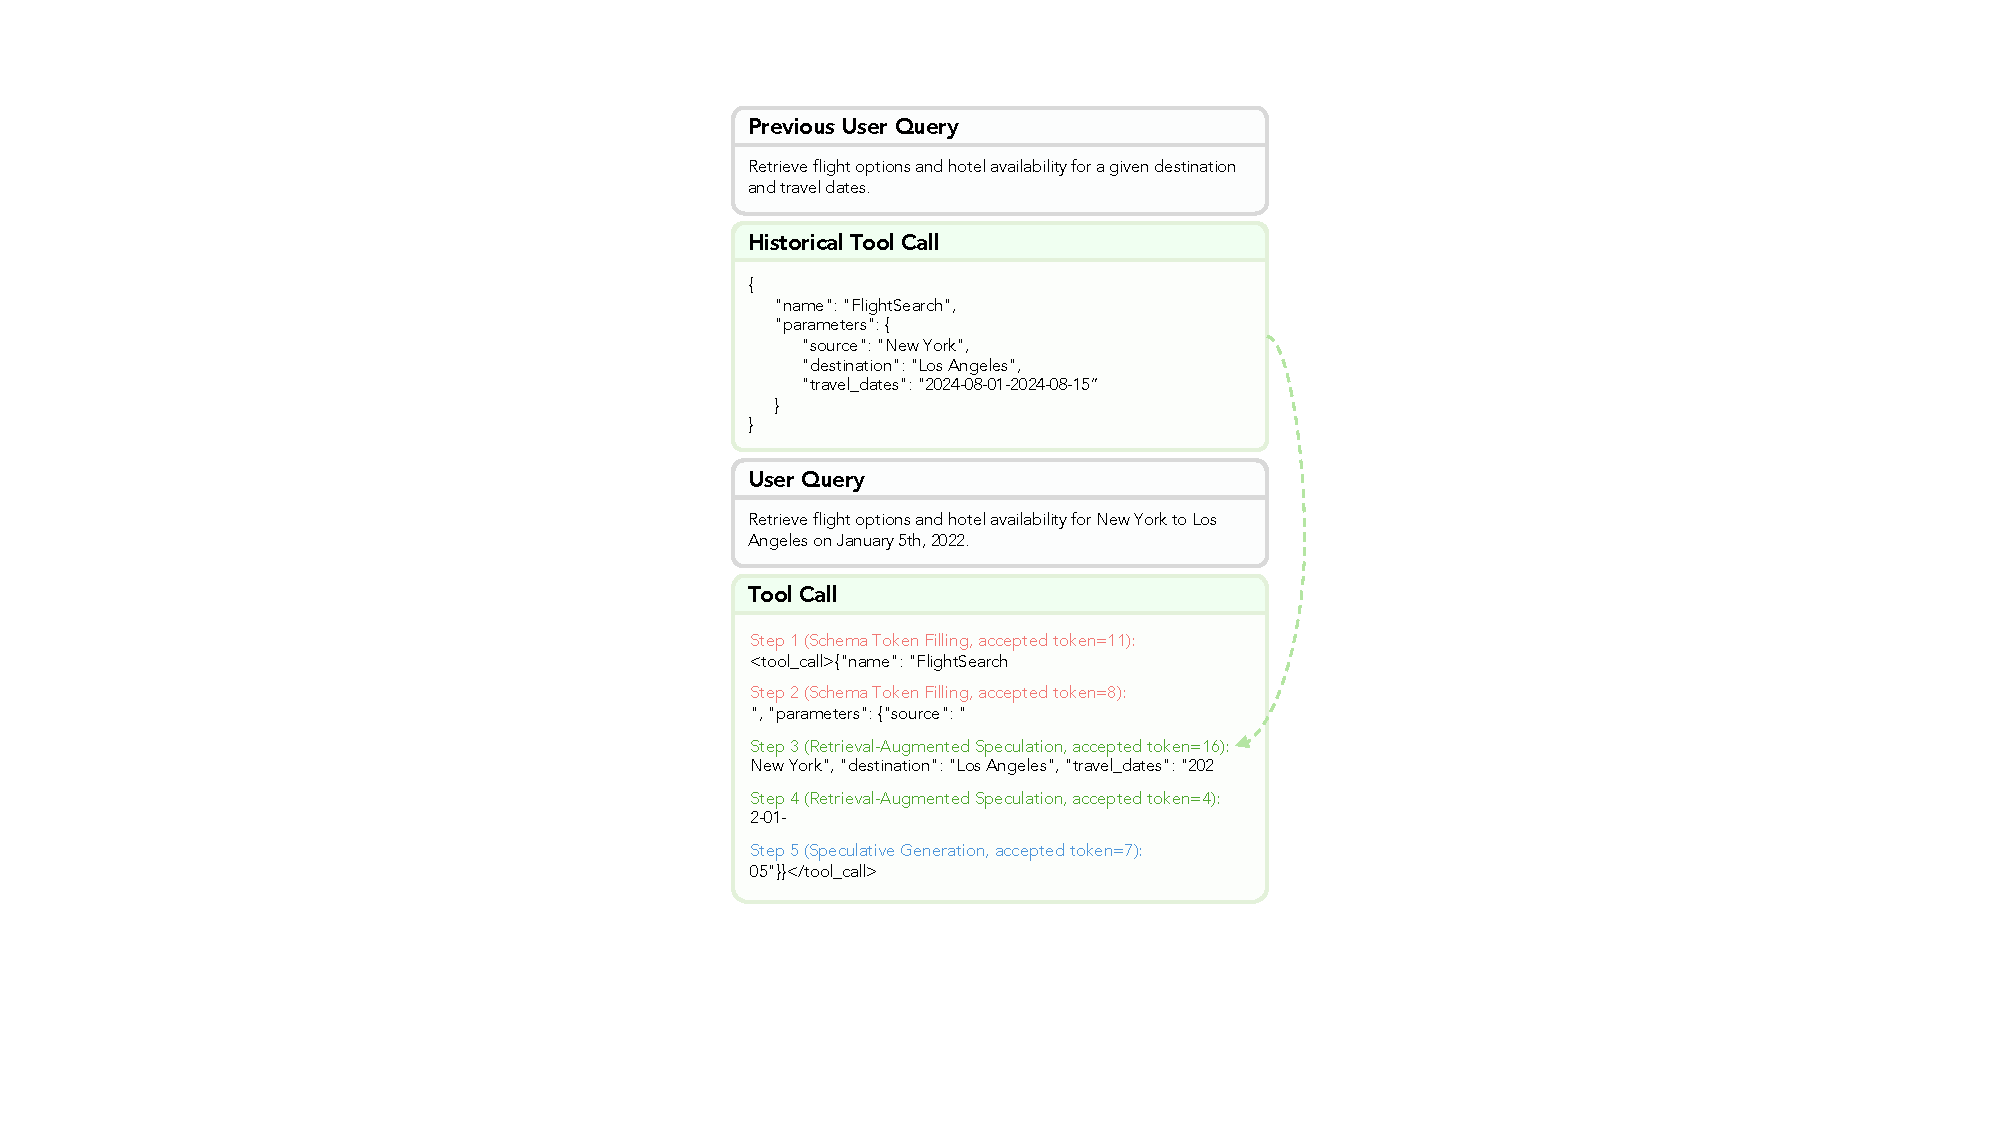
\includegraphics[width=0.95\columnwidth]{fig/case2.pdf}
\caption{Case study of \method under different tool-argument values using LLaMA-3.1-8B-Instruct.}
\label{fig:case2}
\end{figure}

\subsection{Case Study}
Figure~\ref{fig:case1} presents a case study of \method on API-Bank using LLaMA-3.1-8B-Instruct, where the current user query is similar to previously observed queries. As shown, \method first applies schema token filling to generate the required tool name and schema-constrained tokens. It then retrieves a highly similar historical tool call and reuses its continuation as draft tokens, yielding up to 33 accepted tokens in subsequent decoding steps. This case demonstrates the effectiveness of schema token filling and retrieval-augmented speculation.

Similarly, Figure~\ref{fig:case2} presents a case with similar user queries but different tool-argument values. \method reuses the continuation of a previous output as draft tokens, yielding 16 accepted tokens in the third decoding step. It then corrects the user-specific travel information and completes the tool call through general speculative generation. This case highlights the strength of \method in repeated tool-calling scenarios, where most tokens can be drafted from historical invocations while the target LLM focuses on key argument values.